\chapter{Method 3: knowledge-driven analysis}
\chaptermark{Knowledge-driven analysis}
\label{chap:knowledge}
\graphicspath{{./chapters/5-knowledge/figs/}}

% Introduction
\section{Introduction}
\label{sec:kn:introduction}
% more detail in the thesis of Clement

In this section, we introduce an unsupervised framework for understanding comic book images, based on expert system and knowledge base.
We also detail its application to understanding comics.
Developed in collaboration with Clement...

TODO

\section{Expert system} % (fold)
\label{sec:kn:expert_system}

The purpose of the expert system is to interact with the low level (image processing) iteratively to progressively understand the content of an image, moving from simple to more complex elements.
This approach is similar to~\cite{Sciascio2011Structured} except that in our case the definition of the complex object is not a composition of simple objects but context-driven.

In our system, the expert system includes two models, one formalizing the raw data from algorithms (\emph{Image model}) and the other modelling the domain knowledge of the comic books (\emph{Comics model}).
These two models are ontologies that work together to
%This knowledge is formalized in an ontology that 
express the relations between the primary elements of a document that can be considered as being stable through all instances of the studied domain (Figure~\ref{fig:kn:generic_expert_system}).
Thus, the expression of the constraints applied both to the elements and their relations have to be specific enough because these constraints will be considered as the reference knowledge for the detection of potential errors of the low-level extraction algorithm output.

%%%%%%%%%%%%%%%%%%%%%%%%%%%%%%%%%%%%%%%%%%%%%%%%%%%
 \begin{figure}[!ht]  %trim=l b r t  width=0.5\textwidth,
   \centering
  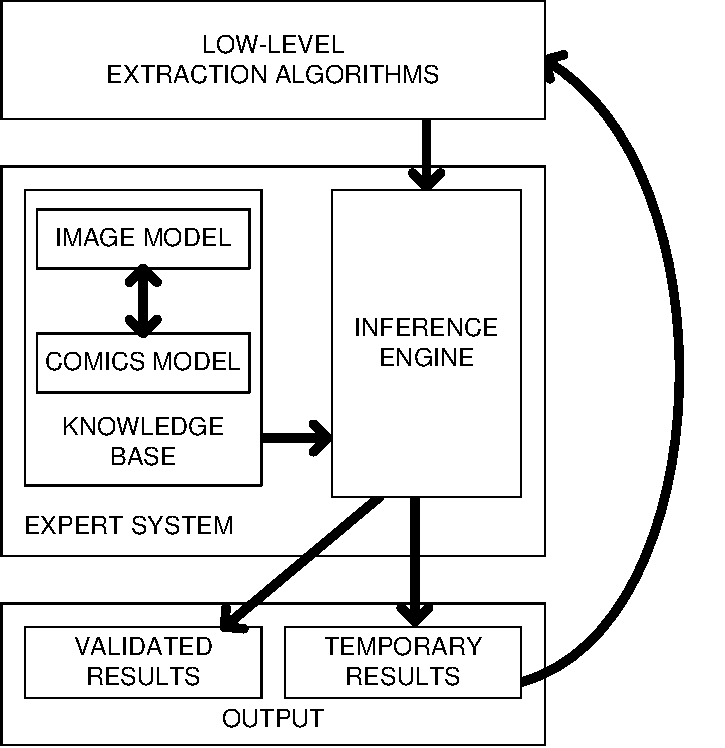
\includegraphics[trim= 0px 0px 0px 0px, clip, width=0.5\textwidth]{expert_system.pdf}
  \caption[Generic representation of the expert system and the relationship between knowledge base, the inference engine and the low-level algorithms]{Generic representation of the expert system and the relationship between knowledge base, the inference engine and the low-level algorithms.}
  \label{fig:kn:generic_expert_system}
 \end{figure}
%%%%%%%%%%%%%%%%%%%%%%%%%%%%%%%%%%%%%%%%%%%%%%%%%%%


%This knowledge can be represented by all the relations betweens the elements that constitute a document from this collection.
The low level algorithms are designed to extract specific information from the whole image or a specific region.
Low and high level systems interact in a loop to feed the knowledge base until there is a complete and consistent understanding of the document, according to the knowledge domain. 
% This loop can be summarized as follows:


%%%%%%%%%%%%%%%%%%%%%%%%%%%%%%%%%%%%%%%%%%%%%%%%%%%
 \begin{figure}[!ht]  %trim=l b r t  width=0.5\textwidth,
   \centering
  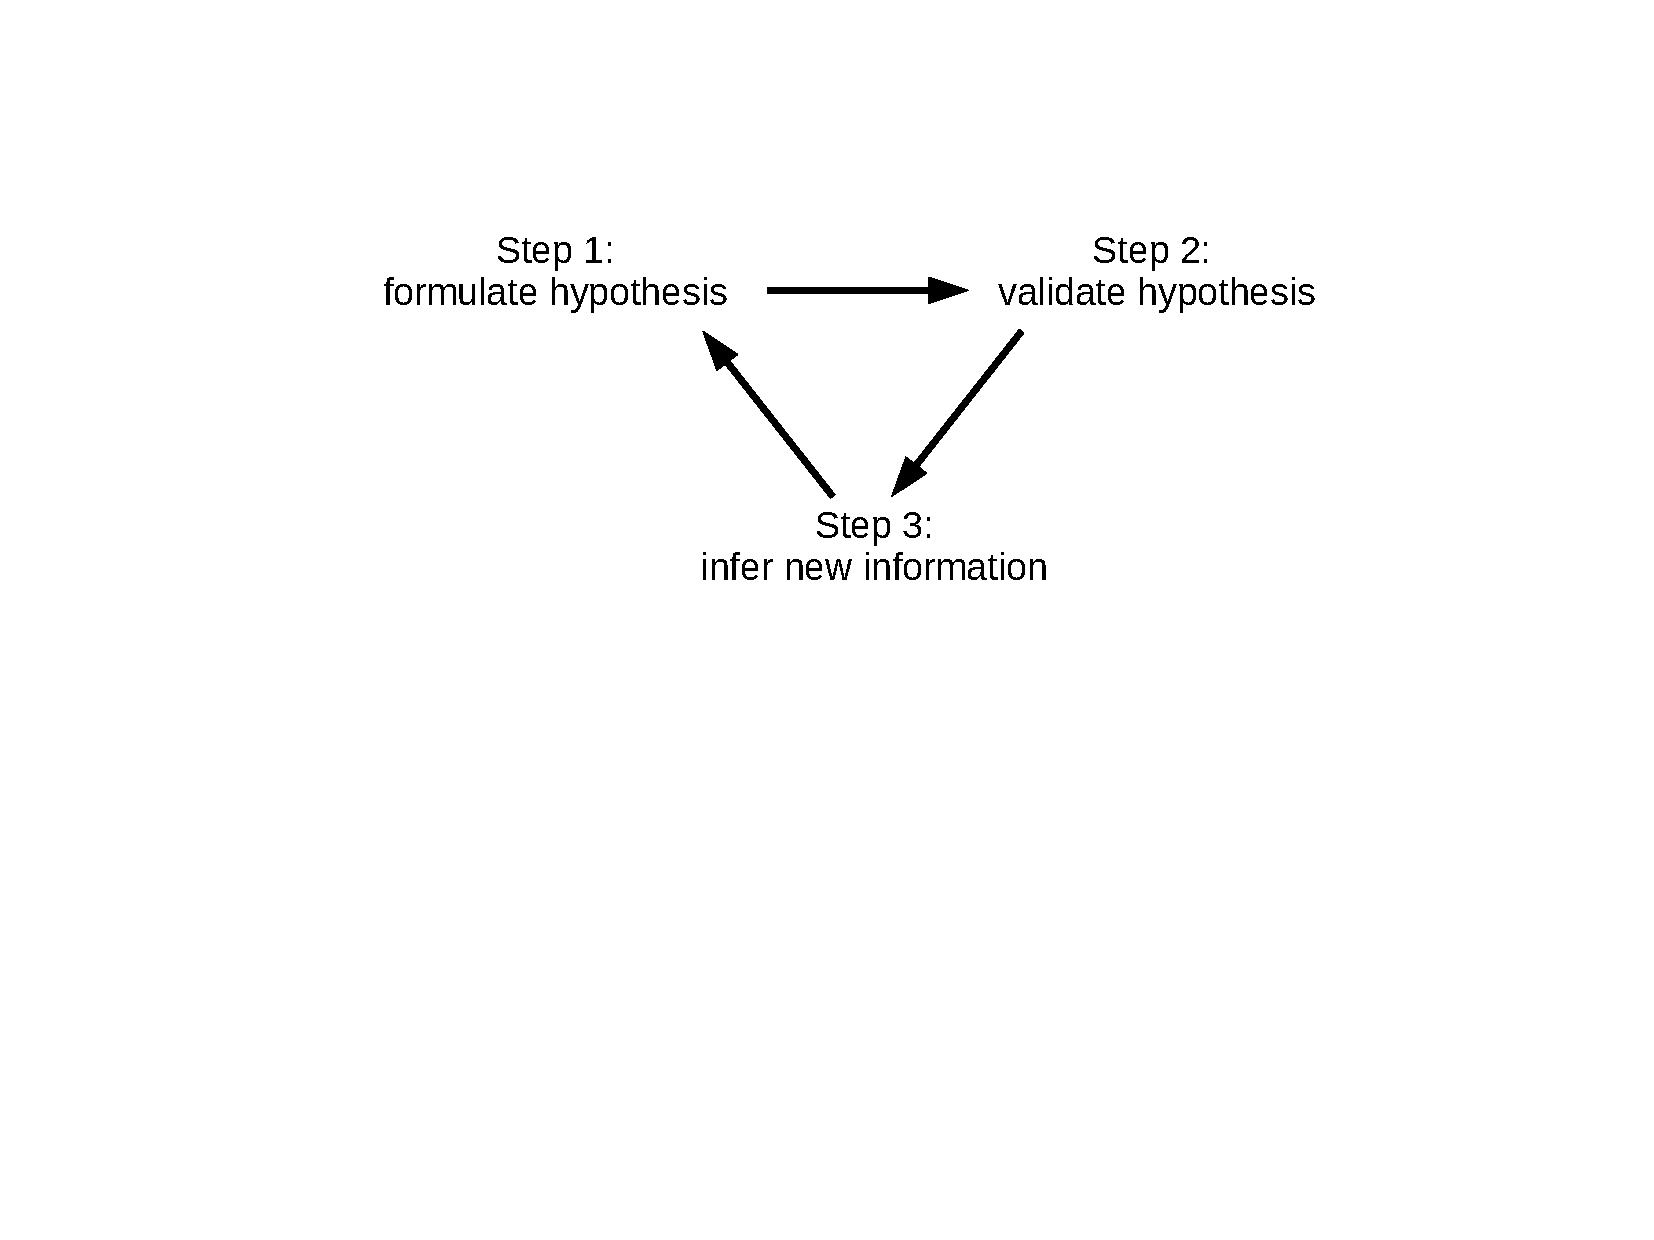
\includegraphics[trim= 140px 350px 100px 95px, clip, width=0.7\textwidth]{process_loop.pdf}
  \caption[Process loop of the knowledge-driven system]{Process loop of the framework.}
  \label{fig:kn:process_loop}
 \end{figure}
%%%%%%%%%%%%%%%%%%%%%%%%%%%%%%%%%%%%%%%%%%%%%%%%%%%

In Figure~\ref{fig:kn:process_loop}, the starting point is step 1 (formulate hypothesis) where low level processing give basic information to the expert system (populating).
%, preferably with a high recall.
Then, step 2 (validate hypothesis) assesses the valid elements and removes obvious mistakes, and in step 3 we infer new information based on the previous information and the knowledge base.
In the next iteration of the process loop, the newly validated information can be used by low level processing (e.g. new parameters, region of interest) to extract more complex elements from the image and so on.
This loop can be run as many times as new information is discovered (until being idempotent).
% section expert_system (end)

\section{Knowledge representation} % (fold)
\label{sec:kn:knowledge_representation}
In our system, knowledge is modelled though the categorization of each element composing a page, combined with a set of topological relation with these elements.
In our context, the elements that compose a given image $I$ are panels $P$, balloons $B$, tails $Q$, text $T$ and characters $C$, as well as the set of topological relations between them.
Because comics, as an art form, do not follow any strict specifications it is really hard to build a perfect model which is valid for all kinds of comics.
There are some instances of comic books without balloons or without panels.
If webcomics are also considered, then a comic is not even necessarily composed of pages.
A model that would be true for every type of comic book would be too general to be of any use in this work.
Instead we define a general comic book model with more constrained properties that represent a large subset of comics (Franco-Belgian, Japanese, American).
The main advantage is that it can be adapted to any kind of document images by defining properties according to the application domain.
We define the general properties of comics as follows:

\begin{itemize}
  \item A panel $P$ is related to one and only one comics page
  \item A balloon $B$ is related to one and only one panel
  \item A character $C$ is related to one and only one panel
  \item A same character can appear only once in a panel
  \item A text line $T$ is related to one and only one balloon $B$
\end{itemize}

Despite the fact that authors are entirely free in their layout choices, some researchers insist a few conventions, widely adopted by comic book' authors, be respected to avoid the reader being confused\cite{Laine2010,Duc1982}.
The depicted elements and their place in the layout must be clearly identifiable at first sight, meaning, for instance, that balloons and characters should be included inside panels.
Whereas one can find some instances of balloons breaking out of their frame, these are usually kept to a minimum.

Therefore, the term ``related'' refers to the situation where an object is overlapped (a fortiori, contained) by another over a \emph{significant} proportion of its surface.
% refers to the smallest region (panel, balloon or text line) covering the object on more than a predefined proportion of its size.
In the case of multiple intersections, only the smallest container is considered.
When the element is fully contained in several other items, the smallest container is consequently the direct container (e.g. a text line must be considered as being included inside a balloon before being included inside the panel containing that balloon).
Considering the lack of accurate numbers on the overlapping ratio of comic book' elements in the literature, we estimated statistically what this \emph{significant proportion} would be using the eBDtheque dataset~\cite{Guerin2013}.
%That proportion depends on the nature of the object as the rules of positioning may vary from a type of element to another.
%We introduce four thresholds that respectively stand for these values for panels, balloons, text lines and characters.
%They have been fixed empirically by monitoring the compliance of our reference dataset to the model, depending on these thresholds.
Figure~\ref{fig:kn:gtfitting} shows the percentage of panels, balloons, text lines and characters that fit the enumerated constraints, as a function of their covered area.

%%%%%%%%%%%%%%%%%%%%%%%%%%
 \begin{figure}[!ht]  %trim=l b r t  width=0.5\textwidth,
   \centering
  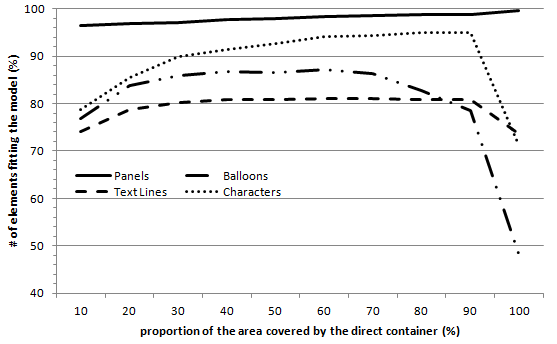
\includegraphics[width=0.8\textwidth]{GTFitting.png}
  \caption[Percentage of panels, balloons, text lines and characters from the eBDtheque dataset that fit the proposed model]{Percentage of panels, balloons, text lines and characters from the eBDtheque dataset~\cite{Guerin2013} that fit the definition given in \ref{sec:kn:knowledge_representation}according to the area proportion that need to be covered.}
  \label{fig:kn:gtfitting}
 \end{figure}
%%%%%%%%%%%%%%%%%%%%%%%%%%

Considering ideal proportion covered for each type of element, we obtained the following overall scores: 99.6\% of the panels, 87.4\% of the balloons, 81.6\% of the text lines and 94.9\% of the characters are in accordance with the assumed constraints in the eBDtheque dataset.
%Table~\ref{tab:related} shows the amount of panels, balloons and text lines from the the eBDtheque dataset that fit these constraints, depending on $T_r$.
%

Semantic relations were also defined in order to categorise some region types such as balloons into speech balloon $SB$ (versus narrative balloons), characters into speaking characters $SC$ (versus non-speaking characters) and text lines as speech text $ST$ (versus narrative lines):
\begin{itemize}
  \item A $SB$ is a balloon $B$ that has a tail and contains text
  \item A $SC$ is a character $C$ pointed by a tail
  \item A $ST$ is a text line which is included in one speech balloon
\end{itemize}

The term ``pointed'' refers to the fact that the character is included in the part of the panel indicated by the tail. To have a better understanding of how a panel is divided according to tail direction, please refer to Section~\ref{sec:se:tail_to_character}.

% The semantic links between speech text and speech balloon are called $STSB$ and the ones between speech balloon and speaking character $SBSC$, they characterise a dialogue.
% They are considered as being true or false according to their existence or not in the ground truth.
% We evaluate the semantic relations $STSB$ and $SBSC$ according to the metadata in the ground truth of eBDtheque dataset~\cite{Guerin2013} called \emph{isLineOf} and \emph{isSaidBy}, which represent 3427 and 880 relations respectively.
% Given the panel, balloon and character position from the ground truth, the accuracy of the expert system to predict the semantic relations is about 96.9\% for $STSB$ and 70.66\% for $SBSC$.

% The 3.1\% of missed \emph{isLineOf} relations
% %that do not fit the proposed model ($\approx$3\%) 
%  are coming from balloons that are not compliant with our model.
% %included in other text lines bounding boxes (e.g. a page number in the corner of a big text region such as the page title).
% In the same way, over the 880 \emph{isSaidBy} relations, that link speech balloons to speaking characters, 9.5\% are undetectable because generated from balloons outside of any panels.
%also coming from uncompliant balloons that are not compliant with our model.
% To have a better figure on the performance of the speaker and spoken text lines inference system, we shall isolate the potential error sources.
%\modif{Reported on 796 identifiable \emph{isSaidBy} relations, the performance of the expert system to identify speaking characters rise up to 80.9\%, while spoken text line inference reach almost 100\%.}

These figures represent the theoretical limit that can be reached with the model in terms of component extraction performance.
% section knowledge_representation (end)

\section{Processing sequence} % (fold)
\label{sec:kn:framework_}
The expert system asserts the extraction of simple elements such as panels, texts, balloons and tails in order to infer speech balloons before searching for more complex elements (e.g. comic book characters) based on the context defined by the simple elements and their relations.
This can be demonstrated with the first two iterations of the process loop as shown in Figure~\ref{fig:kn:process_loop}.
These sections are detailed bellow.
% The details of the two iteration process used here is described in table~\ref{tab:two_iteration}.% decomposed as follows:%in the global loop process:


%%%%%%%%%%%%%%%%%%%%%%%%%%%%%%%%%%%%%%%%%%%%%%%%%%%
%   \begin{table}[ht]
%     \normalsize
% %\renewcommand{\arraystretch}{1.2}

%     \centering
%     \caption{Detail of the two iterations process.}
%     \setlength{\tabcolsep}{.45em}
%     \begin{tabular}{|c|c|c|c|}
%           %\hline
%           %    & \multicolumn{2}{|c|}{P}   & \multicolumn{2}{|c|}{B} & \multicolumn{2}{|c|}{SB}& \multicolumn{2}{|c|}{C} & \multicolumn{2}{|c|}{SC}  \\
%           \hline
%           Ite. &  Hypothesis  & Validation &  Inference      \\
%           % \hline
%           % Before validation   & ?   & ?           \\
%           \hline
%           1  
%           & \begin{tabular}[x]{@{}c@{}}Panel\\Text\\Balloon\end{tabular} 
%           & \begin{tabular}[x]{@{}c@{}}Panel\\Text\\Balloon\end{tabular}  
%           & \begin{tabular}[x]{@{}c@{}}Speech balloon\\Spoken text\\Link text/balloon\end{tabular}             \\
%           \hline
%           2  & ROI character   & Character  & \begin{tabular}[x]{@{}c@{}}Speaking character\\Link balloon/character\end{tabular}             \\
%           \hline
          
%           % TOTAL   & 93.4    & 92.8          \\
%           % \hline
%         %       Proposed multi scale & ???  &???  & ???   & ???       \\
%         %   \hline
%         \end{tabular}
%     \label{tab:two_iteration}
%   \end{table}%
    %%%%%%%%%%%%%%%%%%%%%%%%%%%%%%%%%%%%%%%%%%%%%%%%%%%

\paragraph{Iteration 1 - step 1 (hypothesis)} % (fold)
\label{par:step_1}
The initial extraction of panels, text and balloons feeds the knowledge base.
All the elements are extracted independently using the method proposed Chapter~\ref{chap:independent}.
% given an hypothesis on the labels of each region according to the extractor it is from (e.g. for a region from the balloon extractor, the hypothesis is a balloon label).
In Figure~\ref{fig:kn:graph0}, dashed elements represent the initial hypotheses.
Note that extraction errors can take place at this stage which the system can recover from at a later stage.
% have been introduced in the example in order to demonstrate how the proposed system can recover them.
% The regions that have been validated by the expert system have a solid border, others a dashed border.


%%%%%%%%%%%%%%%%%%%%%%%%%%%%%%%%%%%%%%%%%%%%%%%%%%%
 \begin{figure}[!ht]  %trim=l b r t  width=0.5\textwidth,
   \centering
   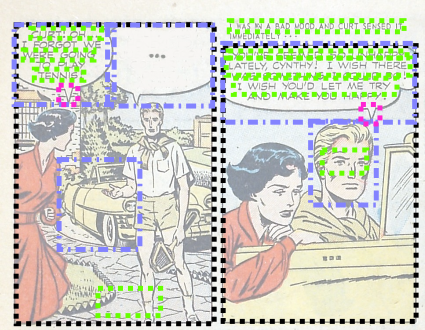
\includegraphics[trim= 0px 0px 0px 0px, clip, width=0.5\textwidth]{process_illustration_hypo_1.png}\\
  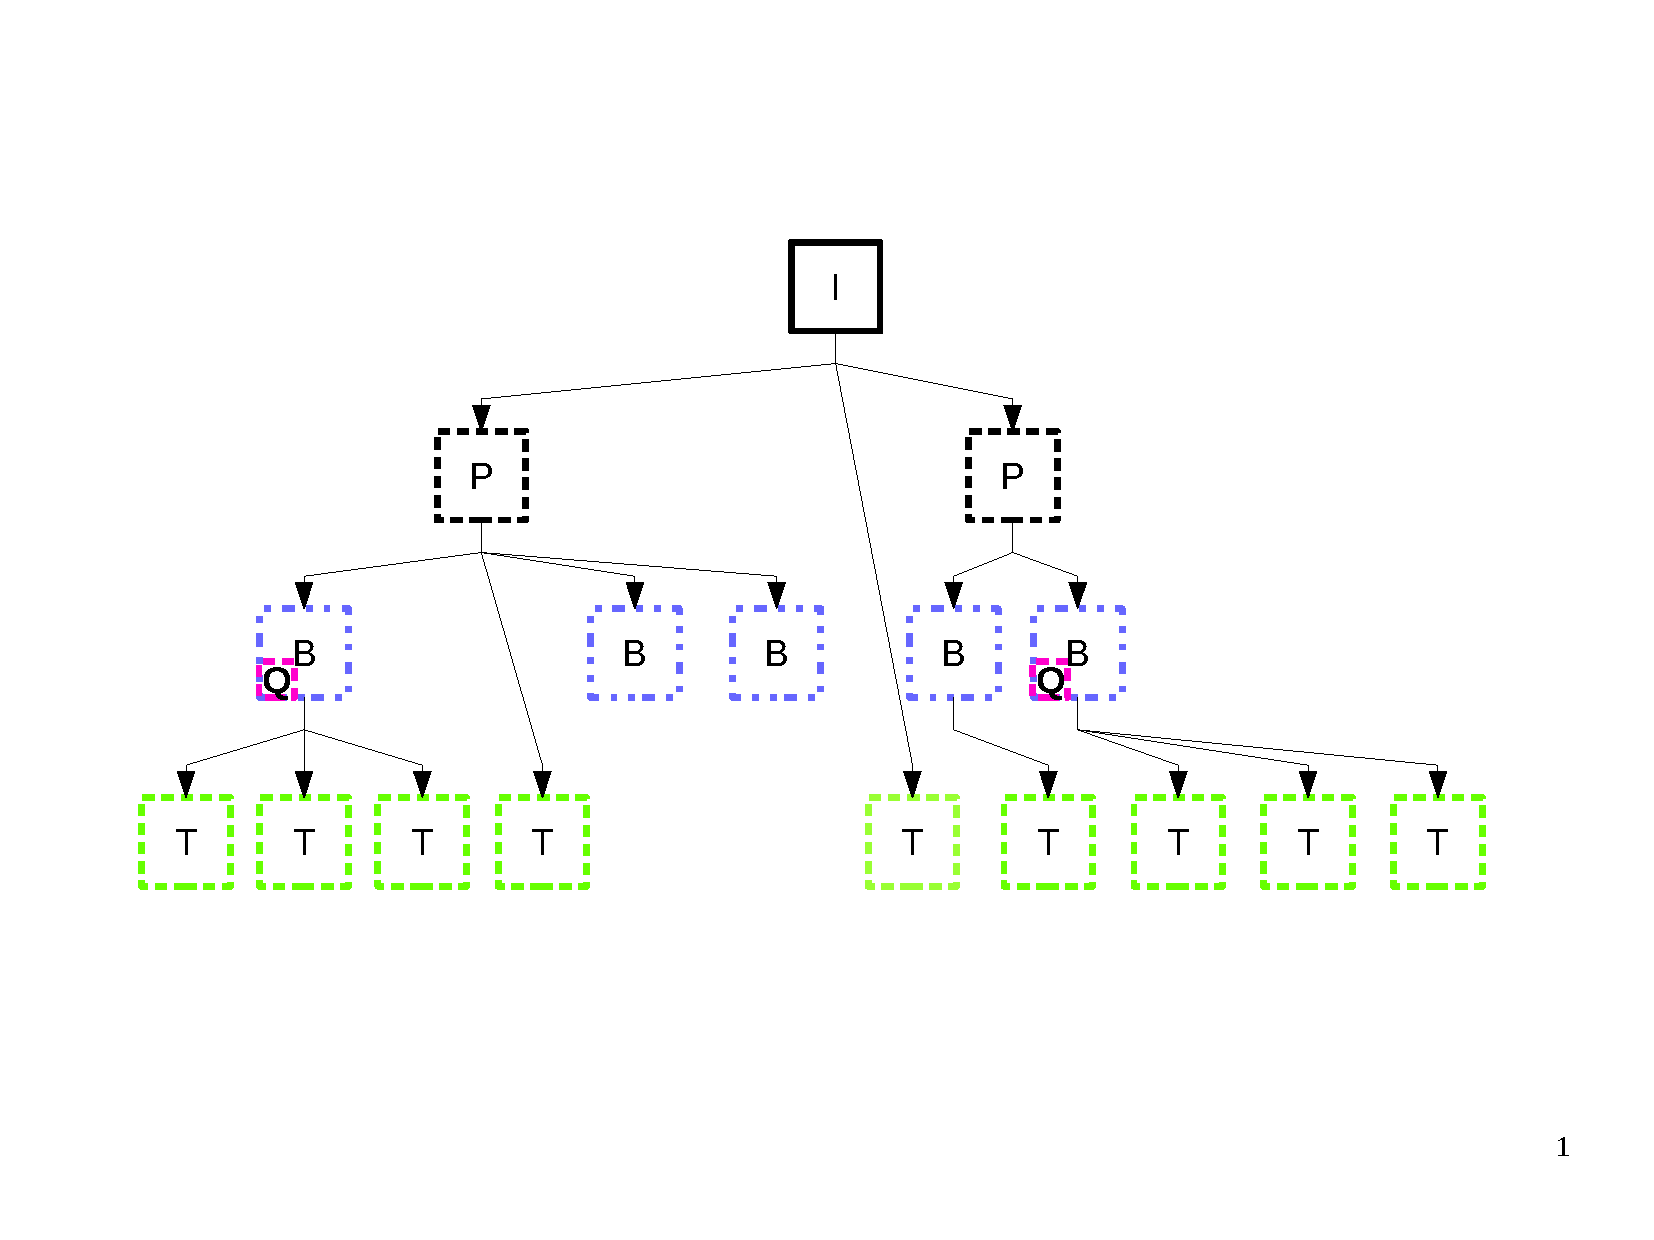
\includegraphics[trim= 30px 168px 20px 110px, clip, width=0.8\textwidth]{graph_init_1.pdf}
  \caption[Initial hypothesis about the content of a given image]{Initial hypothesis (dashed elements) about the content of a given image $I$ after the initial extractions of panels $P$, text $T$ and balloons $B$ with tails $Q$.
  }
  \label{fig:kn:graph0}
 \end{figure}
%%%%%%%%%%%%%%%%%%%%%%%%%%%%%%%%%%%%%%%%%%%%%%%%%%%

\paragraph{Iteration 1 - step 2 (validation)} % (fold)
\label{par:step_2}
Subsequently, the expert system checks if their spatial relations (context) match the topological properties of the knowledge base defined Section~\ref{sec:kn:knowledge_representation}, otherwise it solves them using the domain knowledge described in Section~\ref{sub:kn:validation}.
The result is illustrated in Figure~\ref{fig:kn:graph_valid_initial}.


%%%%%%%%%%%%%%%%%%%%%%%%%%%%%%%%%%%%%%%%%%%%%%%%%%%
 \begin{figure}[!ht]  %trim=l b r t  width=0.5\textwidth,
   \centering
   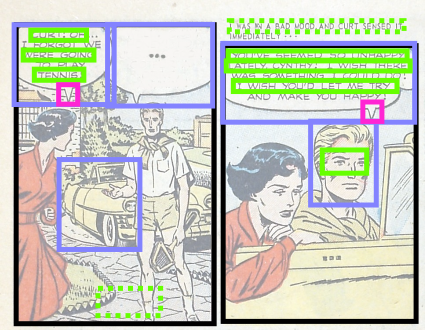
\includegraphics[trim= 0px 0px 0px 0px, clip, width=0.5\textwidth]{process_illustration_valid_1.png}\\
  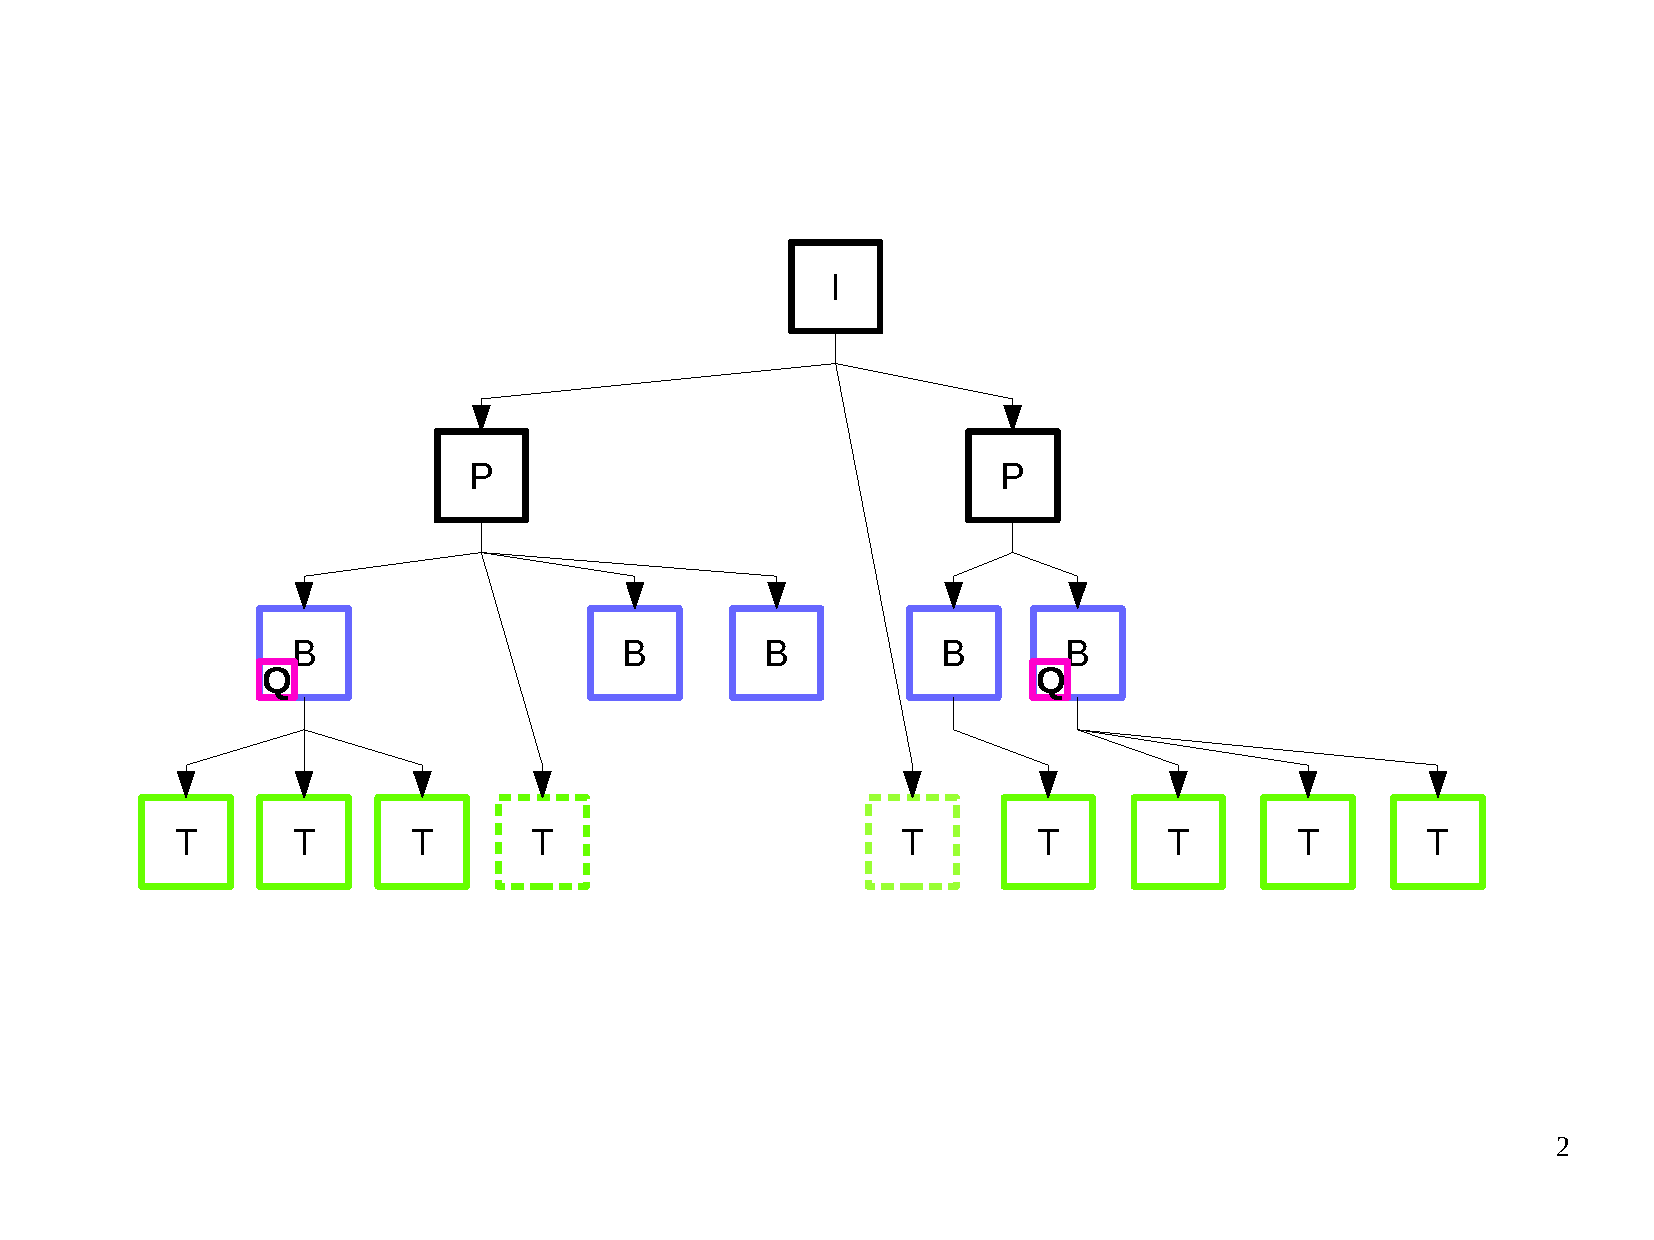
\includegraphics[trim= 30px 168px 20px 110px, clip, width=0.8\textwidth]{graph_valid_1.pdf}
  \caption[Validation of the hypothesis using the properties of the knowledge base]{Validation of the hypothesis using the properties of the knowledge base. Valid elements have a solid border.}
  \label{fig:kn:graph_valid_initial}
 \end{figure}
%%%%%%%%%%%%%%%%%%%%%%%%%%%%%%%%%%%%%%%%%%%%%%%%%%%

\paragraph{Iteration 1 - step 3 (inference)} % (fold)
\label{par:step_3}
From the validated information, the expert system infers the semantic information between text and balloon and specifies them as speech balloon and speech text respectively when they verify the properties of the knowledge base (Figure~\ref{fig:kn:graph_specific_types}). 

%%%%%%%%%%%%%%%%%%%%%%%%%%%%%%%%%%%%%%%%%%%%%%%%%%%
 \begin{figure}[!ht]  %trim=l b r t  width=0.5\textwidth,
   \centering
  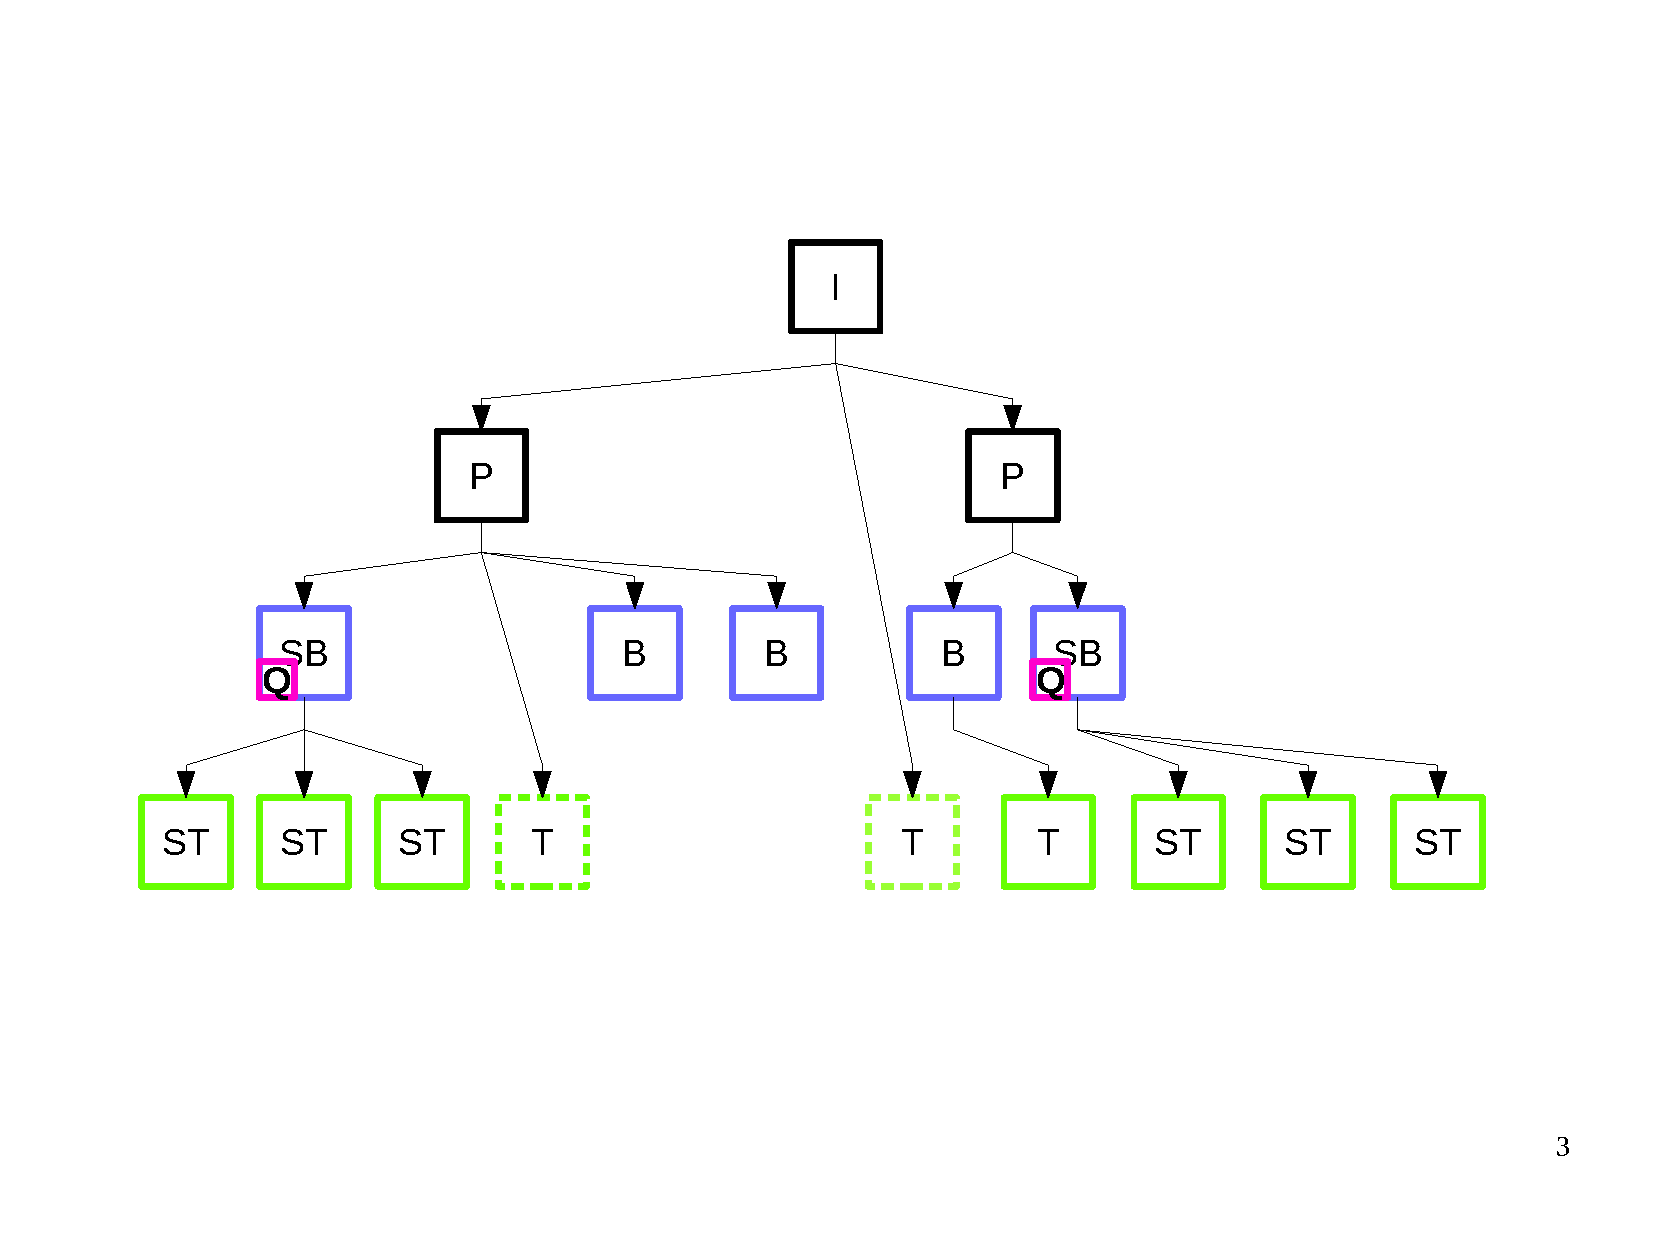
\includegraphics[trim= 30px 168px 20px 110px, clip, width=0.8\textwidth]{graph_infer_1.pdf}
  \caption[Inference of the speech balloon $SB$ and speech text $ST$ regions using the semantic properties of the knowledge base]{Inference of the speech balloon $SB$ and speech text $ST$ regions using the semantic properties of the knowledge base.% Bold edges represent an information spatial and semantic.
  }
  \label{fig:kn:graph_specific_types}
 \end{figure}
%%%%%%%%%%%%%%%%%%%%%%%%%%%%%%%%%%%%%%%%%%%%%%%%%%%

\paragraph{Iteration 2 - step 1 (hypothesis)} % (fold)
\label{par:step_4}
This step is the beginning of the second iteration of the process illustrated Figure~\ref{fig:kn:process_loop}.
At this point the expert system already has some information about the content of the image from which a further hypothesis can be made concerning complex elements such as the region of interest (ROI) of the characters from the speech balloon positions (Figure~\ref{fig:kn:hypothesis_roi}).
The ROIs defined by the expert system are given as seeds to the image processing algorithm (extractor of characters) which in turn feeds the expert system with more precise character locations (Figure~\ref{fig:kn:graph_character_region}).

% Knowing the position of the valid from the valid triplets of panel, text and balloon.
% This is the starting point of the second iteration.

%%%%%%%%%%%%%%%%%%%%%%%%%%%%%%%%%%%%%%%%%%%%%%%%%%%
 \begin{figure}[!ht]  %trim=l b r t  width=0.5\textwidth,
   \centering
   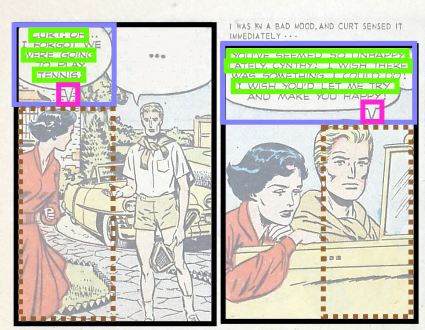
\includegraphics[trim= 0px 0px 0px 0px, clip, width=0.5\textwidth]{process_illustration_hypo_2_1.png}\\
  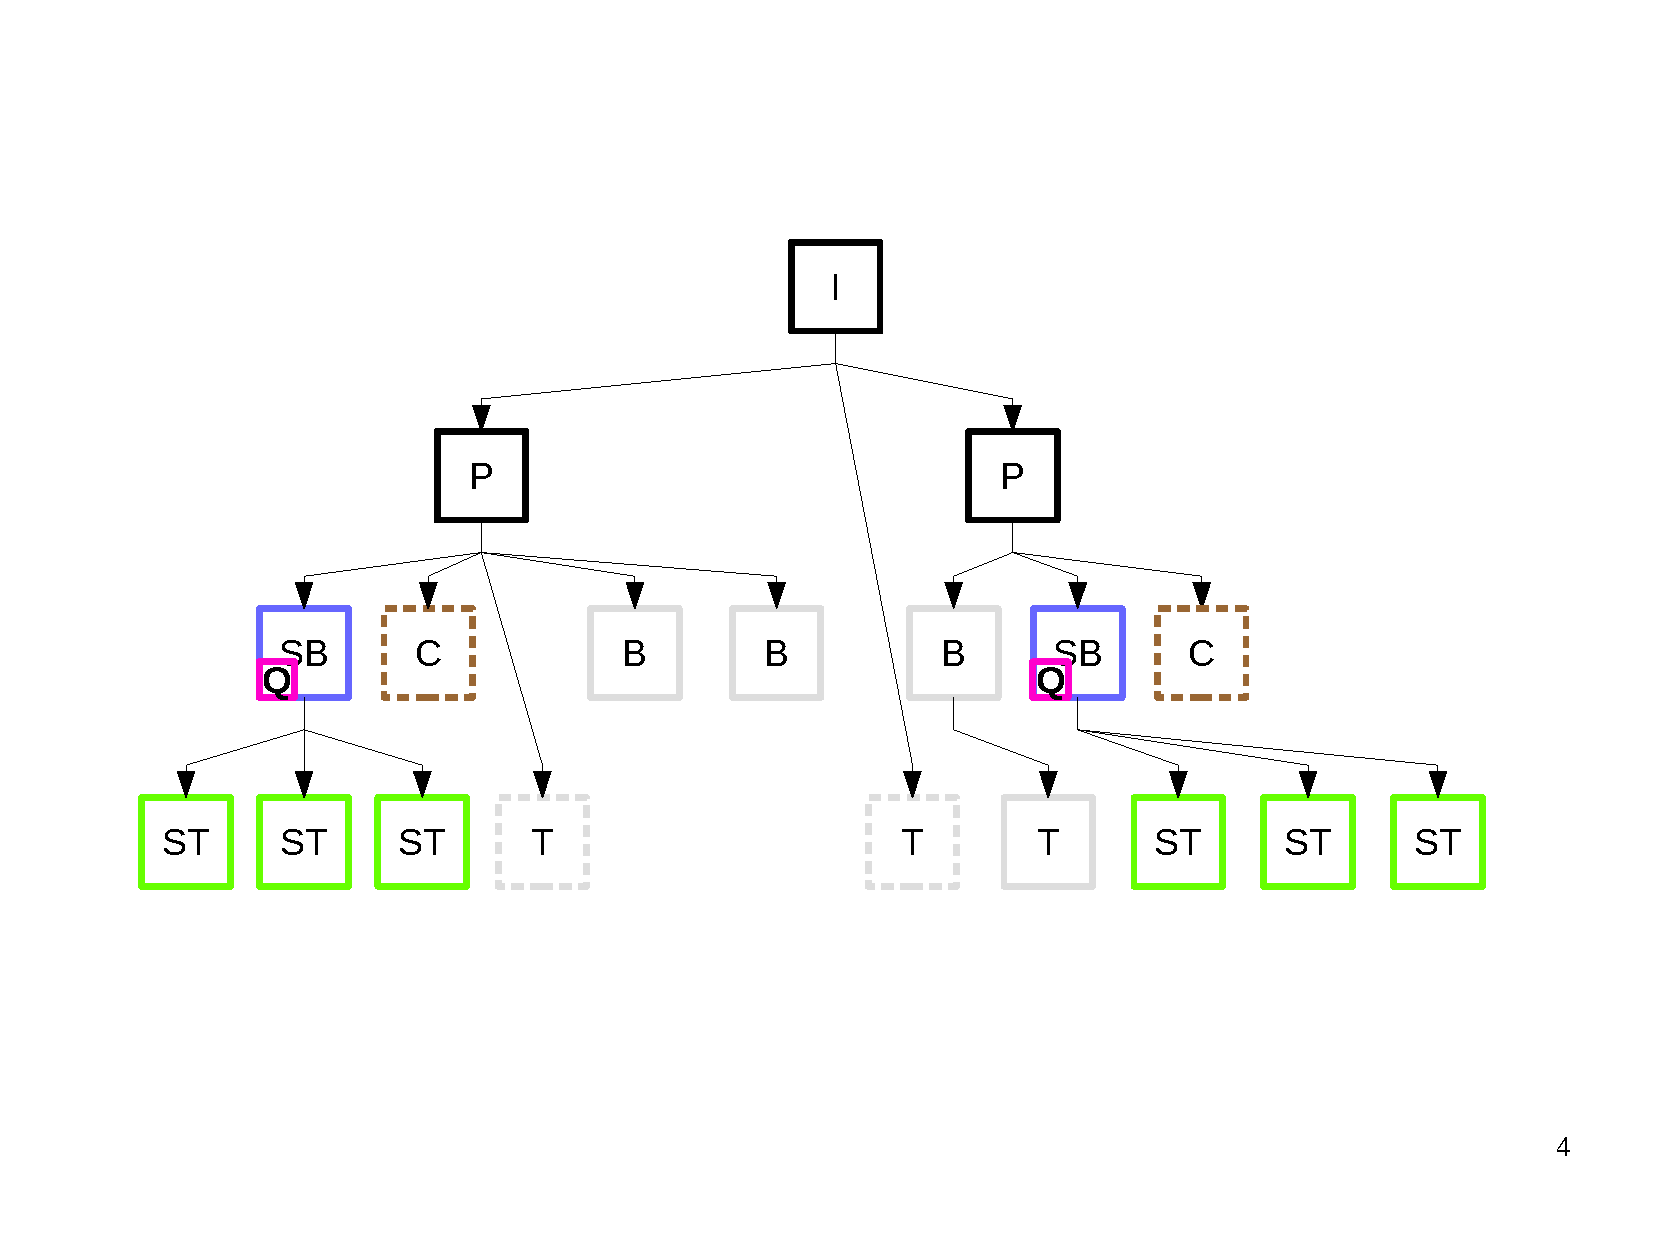
\includegraphics[trim= 30px 168px 20px 110px, clip, width=0.8\textwidth]{graph_init_2_1.pdf}
  \caption[Hypothesis of ROIs of characters $C$ from the speech balloon $SB$ regions and the corresponding image $I$]{Hypothesis of ROIs of characters $C$ from the speech balloon $SB$ regions and the corresponding image $I$. The regions that are not related to $ST$ have been shaded in the graph and removed from the image to make it more comprehensible.
  }
  \label{fig:kn:hypothesis_roi}
 \end{figure}
%%%%%%%%%%%%%%%%%%%%%%%%%%%%%%%%%%%%%%%%%%%%%%%%%%%


%%%%%%%%%%%%%%%%%%%%%%%%%%%%%%%%%%%%%%%%%%%%%%%%%%%
 \begin{figure}[!ht]  %trim=l b r t  width=0.5\textwidth,
   \centering
   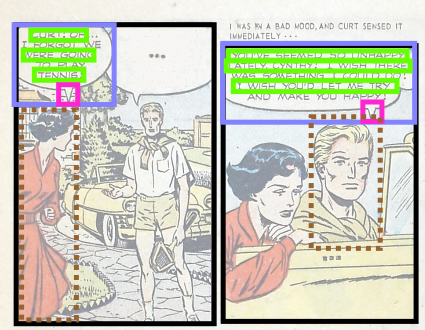
\includegraphics[trim= 0px 0px 0px 0px, clip, width=0.5\textwidth]{process_illustration_hypo_2_2.png}\\
  % 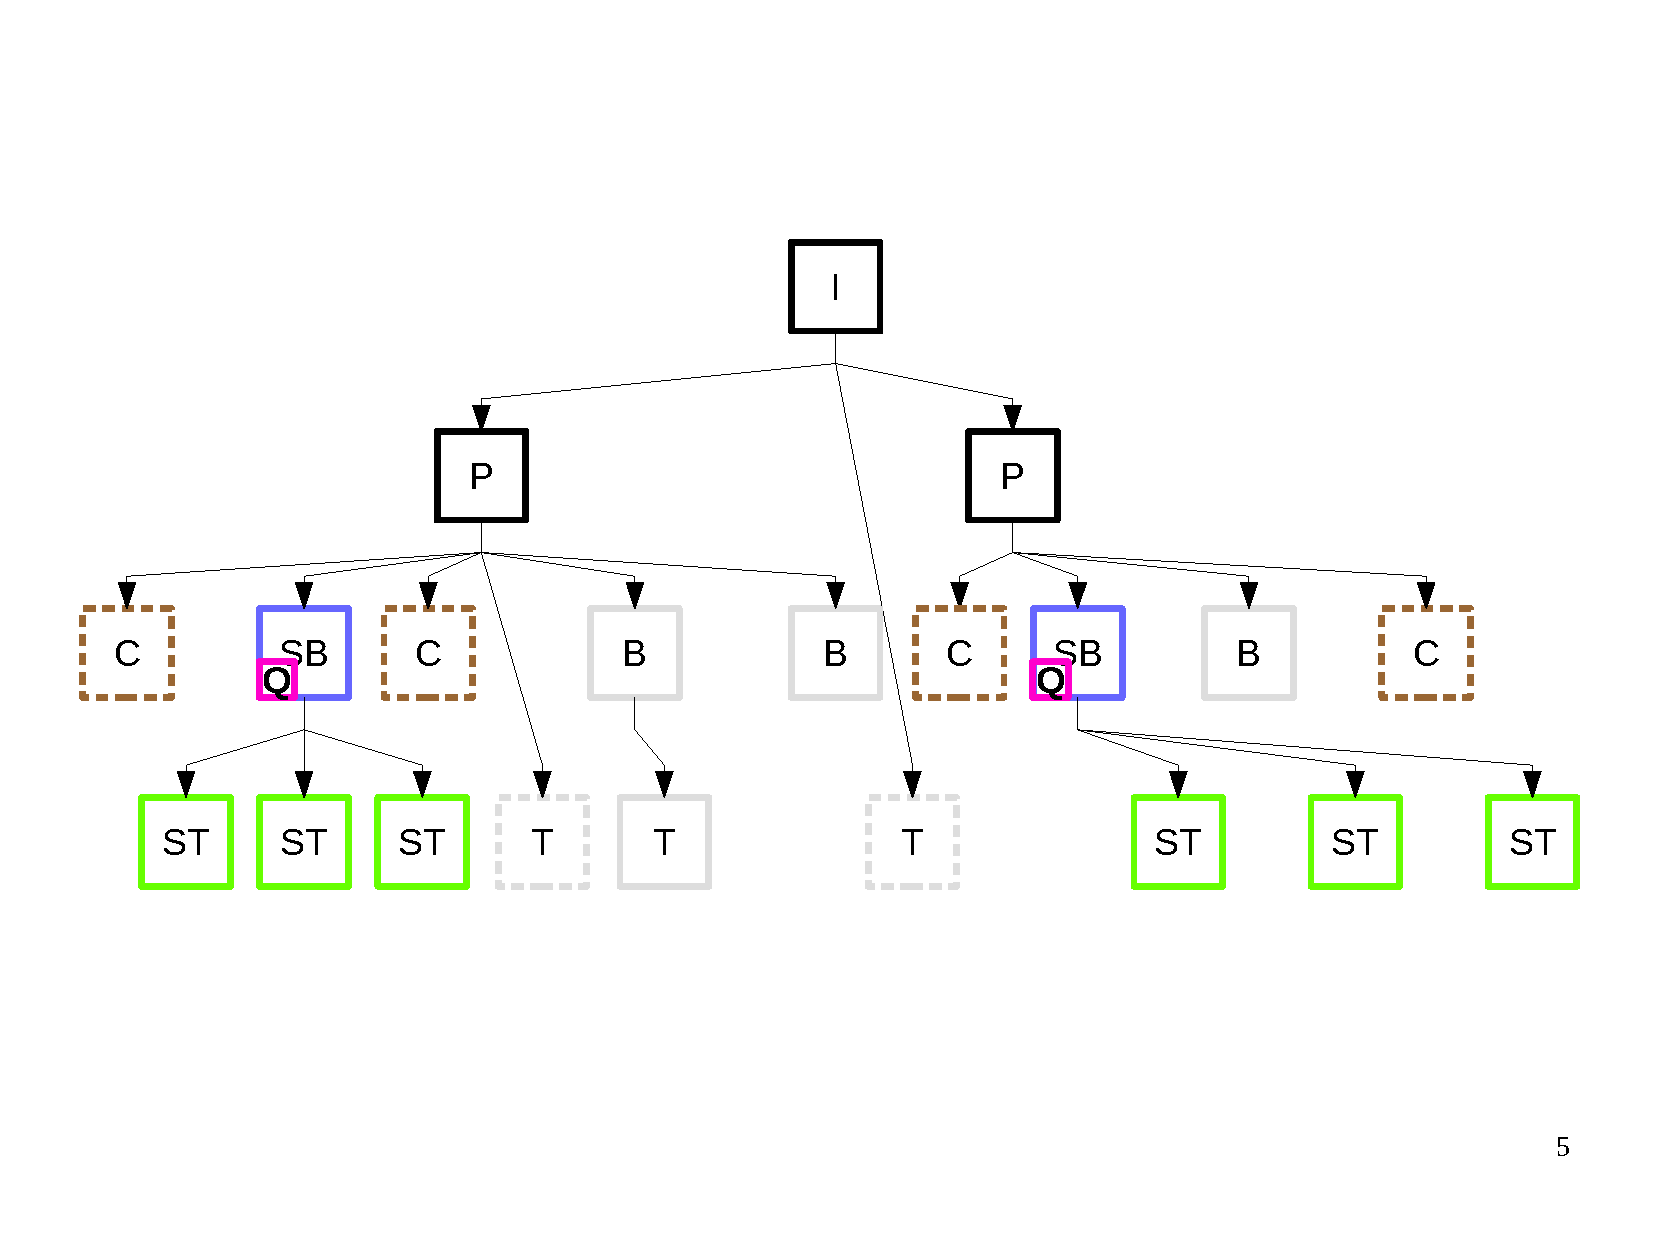
\includegraphics[trim= 0px 168px 20px 85px, clip, width=0.8\textwidth]{fig/graph_init_2_2.pdf}
  \caption[Character locations ($C$) returned by the low level processing]{Character locations ($C$) returned by the low level processing from the ROIs defined in Figure~\ref{fig:kn:hypothesis_roi}.
  }% added into the graph and the corresponding region in the image $I$.}
  \label{fig:kn:graph_character_region}
 \end{figure}
%%%%%%%%%%%%%%%%%%%%%%%%%%%%%%%%%%%%%%%%%%%%%%%%%%%

\paragraph{Iteration 2 - step 2 (validation)} % (fold)
\label{par:step_5}
The expert system checks if the spatial relations of the characters $C$ match the properties of the knowledge base defined in Section~\ref{sub:kn:knowledge_base} (Figure~\ref{fig:kn:valid_2}).


%%%%%%%%%%%%%%%%%%%%%%%%%%%%%%%%%%%%%%%%%%%%%%%%%%%
 \begin{figure}[!ht]  %trim=l b r t  width=0.5\textwidth,
   \centering
   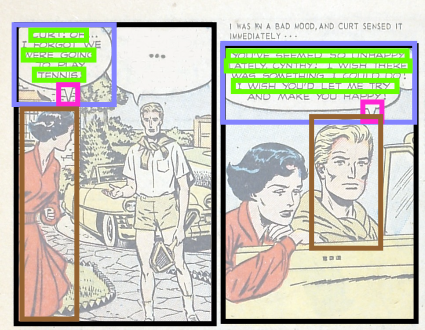
\includegraphics[trim= 0px 0px 0px 0px, clip, width=0.5\textwidth]{process_illustration_valid_2.png}\\
  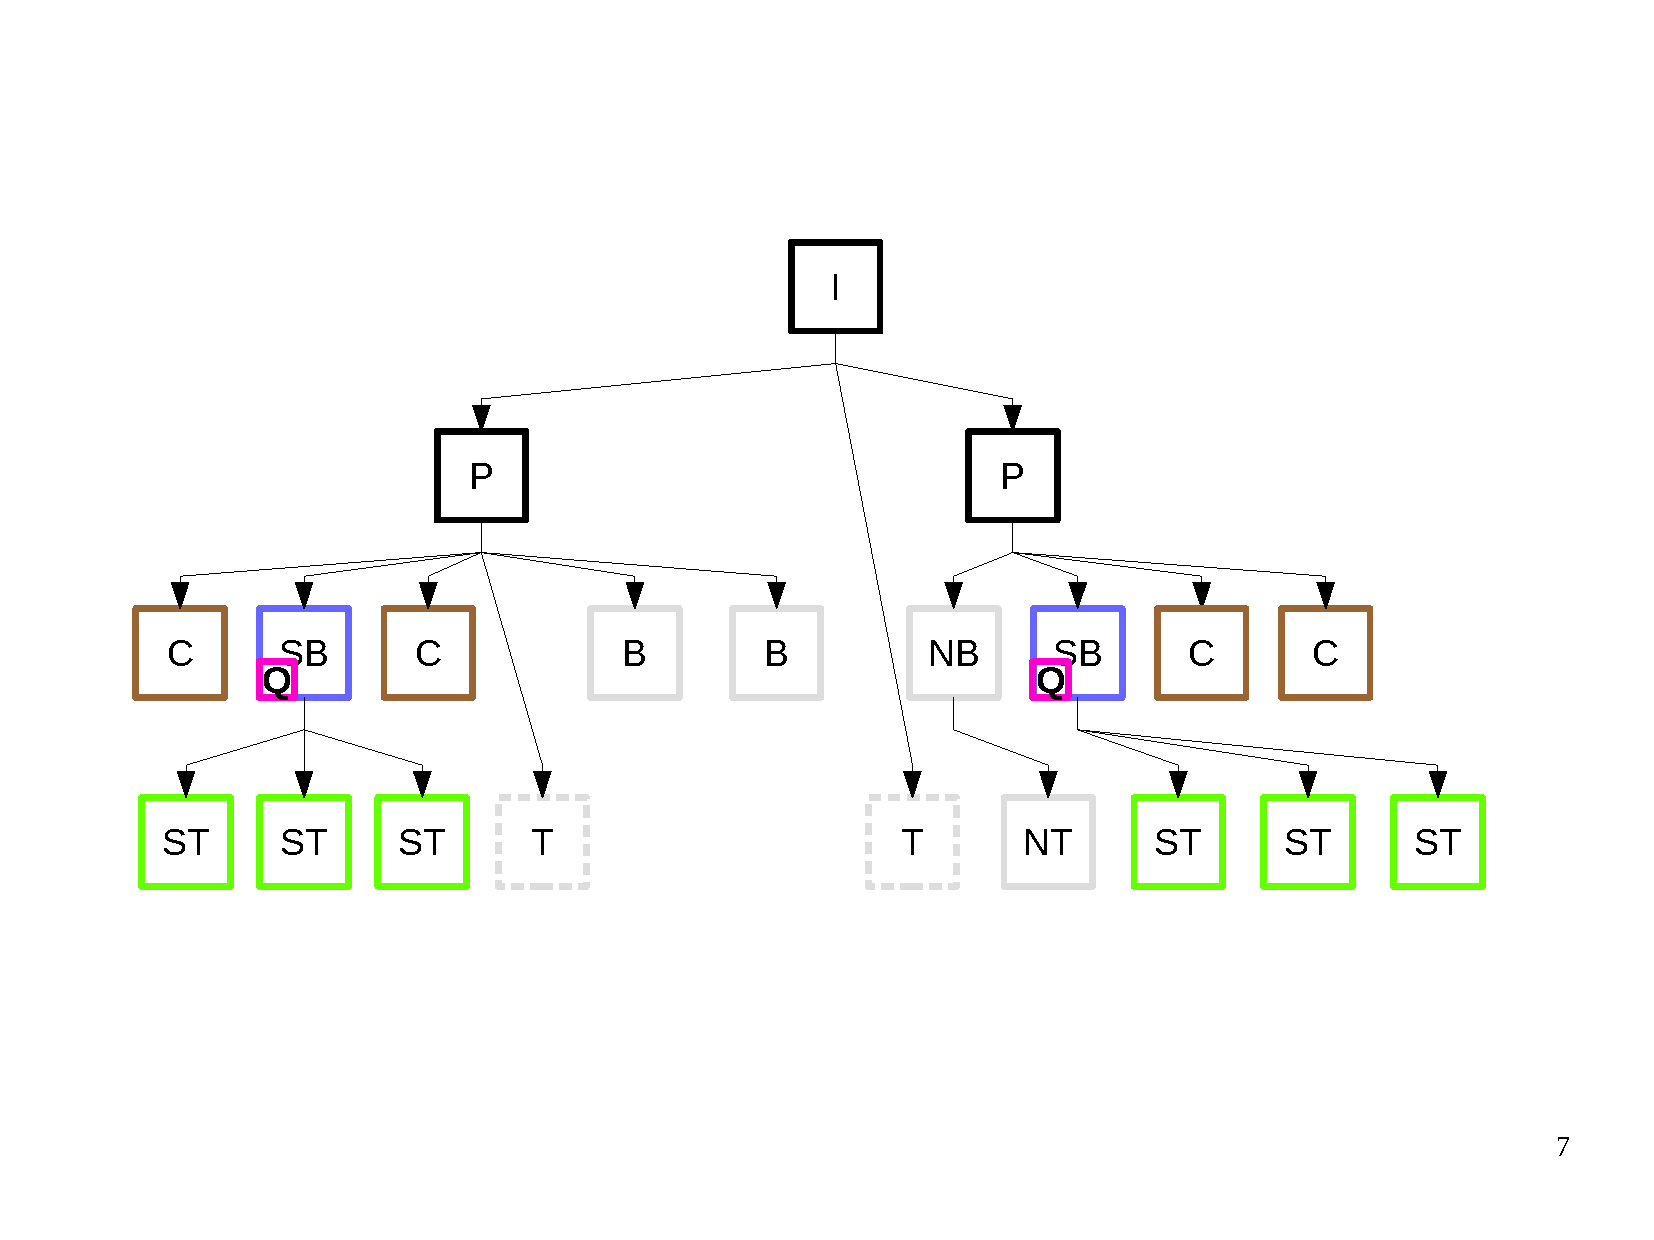
\includegraphics[trim= 0px 128px 20px 85px, clip, width=0.8\textwidth]{graph_valid_2.pdf}
  \caption[Validation of the character regions ($C$) by the expert system]{Validation of the character regions ($C$) by the expert system and the corresponding image $I$.
  }
  \label{fig:kn:valid_2}
 \end{figure}
%%%%%%%%%%%%%%%%%%%%%%%%%%%%%%%%%%%%%%%%%%%%%%%%%%%

\paragraph{Iteration 2 - step 3 (inference)} % (fold)
\label{par:step_6}
The expert system infers which characters are speaking $SC$ (see Section~\ref{sub:inference_of_the_speaking_characters}) and makes a semantic link to the corresponding speech balloons which have already been linked to speech text regions in {\it Iteration 1 - inference} step. (Figure~\ref{fig:kn:final_information}).


%%%%%%%%%%%%%%%%%%%%%%%%%%%%%%%%%%%%%%%%%%%%%%%%%%%
 \begin{figure}[!ht]  %trim=l b r t  width=0.5\textwidth,
   \centering
   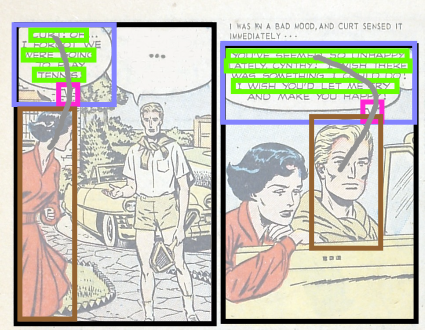
\includegraphics[trim= 0px 0px 0px 0px, clip, width=0.5\textwidth]{process_illustration_infer_2.png}\\
  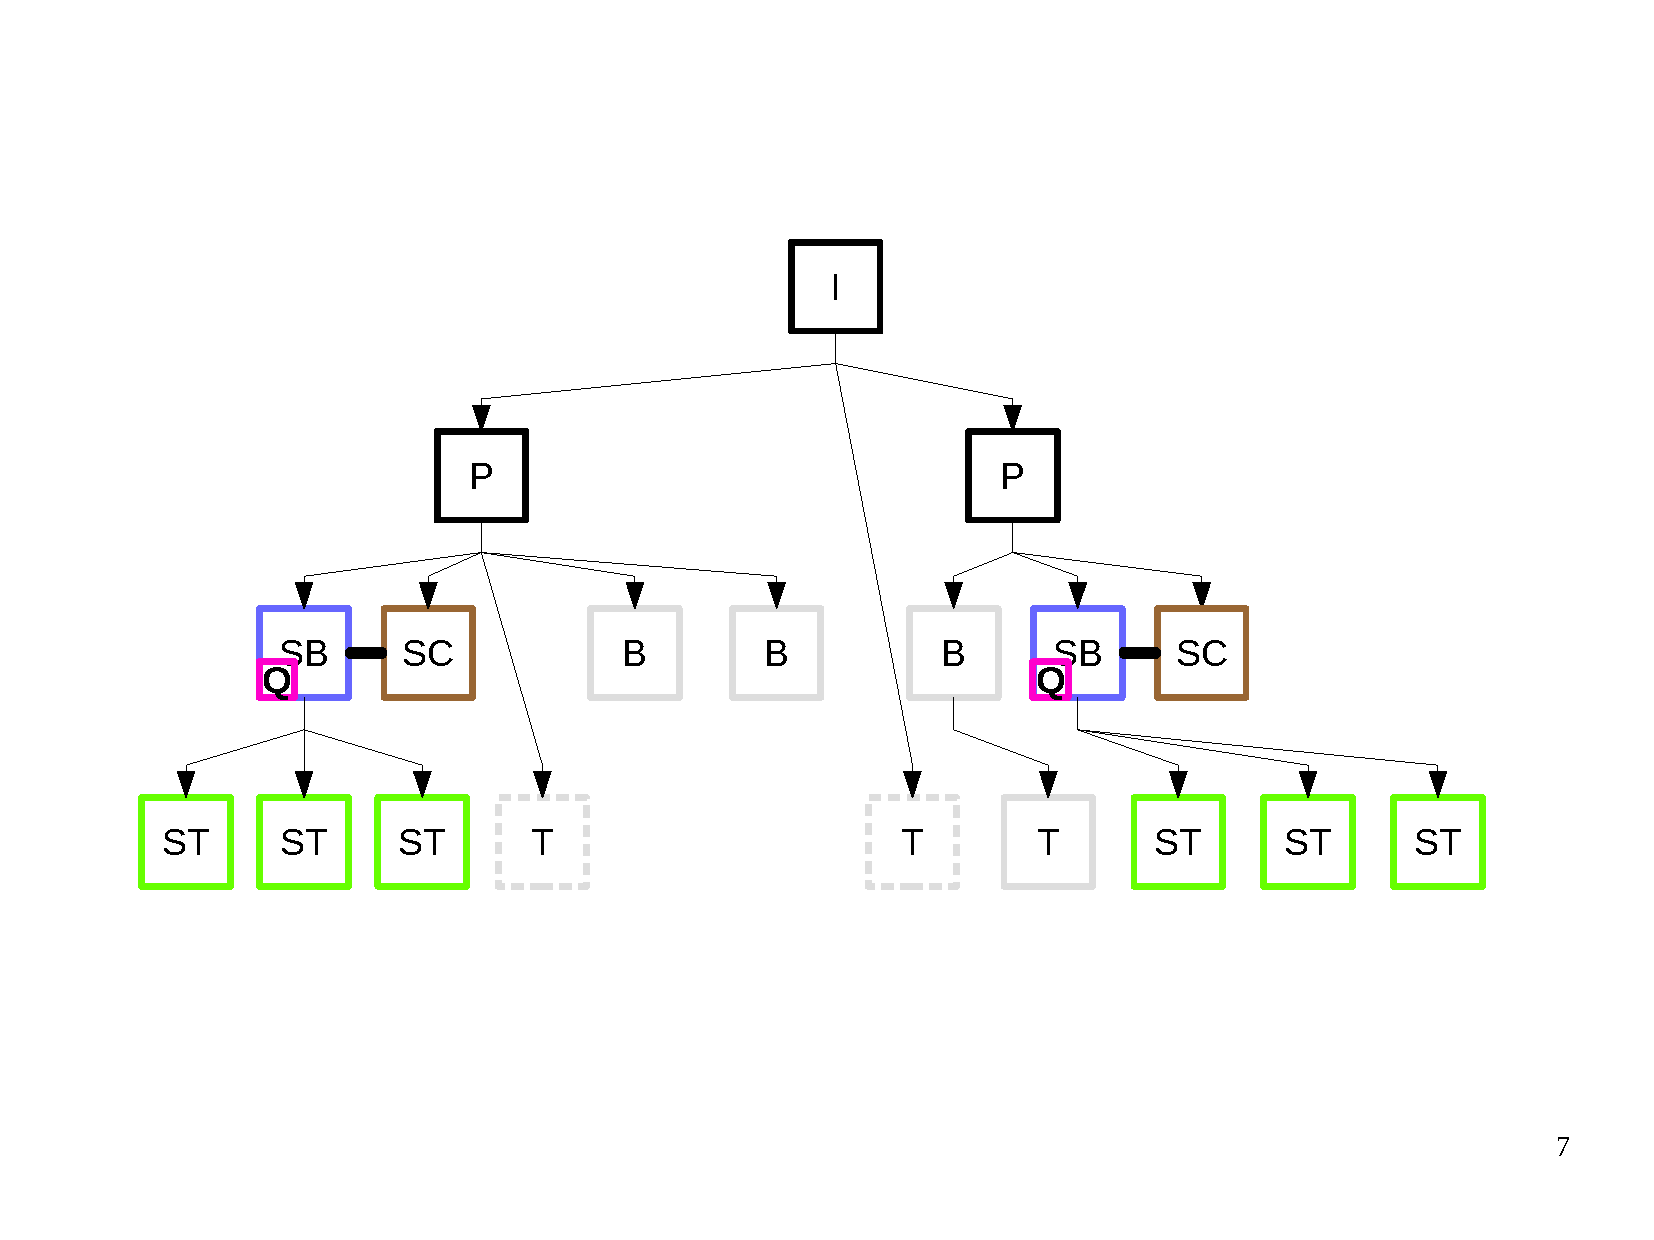
\includegraphics[trim= 0px 128px 20px 85px, clip, width=0.8\textwidth]{graph_infer_2.pdf}
  \caption[Inference of the speaking characters ($SC$) and the corresponding semantic links between speaking characters $SC$ and speech balloons $SB$ regions]{Inference of the two speaking characters ($SC$) and the corresponding semantic links between speaking characters $SC$ and speech balloons $SB$ regions.
  The two semantic links are represented by a grey stroke in the image over the regions concerned and a non oriented horizontal edge in the graph.
  }
  \label{fig:kn:final_information}
 \end{figure}
%%%%%%%%%%%%%%%%%%%%%%%%%%%%%%%%%%%%%%%%%%%%%%%%%%%

At the end of the two iterations we obtained both a topological and a semantic description of the image content, illustrated here in a single graph here.
Further iteration could be processed by extracting other low level elements such as faces or vehicles and by adding extra domain knowledge.

% section framework_ (end)

\section{Presentation of the model} % (fold)
\label{sec:kn:model}

The knowledge base is composed of two ontologies, designed using OWL's W3C recommendation~\cite{McGuinness2004}, and interacting with each other (Figure~\ref{fig:kn:generic_expert_system}).
The first one was used to model the raw data provided by image analysis algorithms (called \textit{image model} hereafter), while the second models the comic book domain knowledge (called \textit{comics model}).
These two models are bounded by bridges that are used to perform reasoning over both models, using their own properties.

\subsection{Image model}
The image model is mostly composed of the concepts of \textit{Image}, \textit{Region of interest (ROI)} and \textit{Extractor}.
It is based on the fact that the output of image analysis algorithms usually corresponds to spatial regions within the image context.
A ROI is necessarily extracted from one and only one image, and by one and only one extractor.
Therefore, the ROI concept is linked to the \textit{Image} and \textit{Extractor} concepts respectively with functional properties \textit{hasImage} and \textit{hasExtractor}.
%Their coordinates are stored in the OpenGIS Well-Know Text (WKT) format \cite{OpenGISConsortiumInc.2011}.

Algorithms may have specific characteristics so they don't produce the same set of regions as the result of the analysis of an image.
Extractors are also usually designed to extract one kind of elements, e.g. panels, balloons, etc.
The purpose of each algorithm is given through the data property \textit{roiType}.
Figure~\ref{fig:kn:model_image} shows a visual representation of these concepts altogether.

 \begin{figure}[!ht]
   \centering
  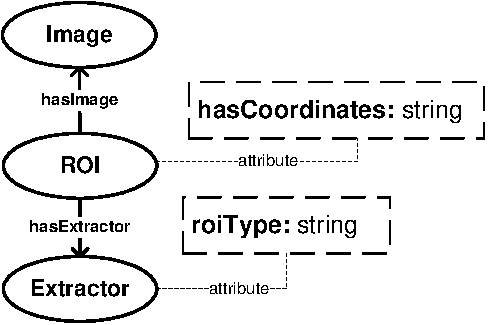
\includegraphics[width=0.5\textwidth]{model_image.pdf}
  \caption[A representation of the image model involved in the expert system]{A representation of the image model involved in the expert system. Concepts are represented by the oval-shaped items, the arrows are the object properties linking them to each other. The dashed rectangles contain the data properties of the concepts they are attached to.}
  \label{fig:kn:model_image}
 \end{figure}

%Moreover, they can be automatic but they also can be manual, if we consider a manual ground truth as a kind of extractor.
%The concept of extractor is extended in two subsumed concepts, \textit{Algorithm} and \textit{GroundTruth}.
%The resulting regions of interest of instances of one of these extractors, are respectively classified as \textit{Automatic regions (ROI\_Auto)} and \textit{Ground truth regions (ROI\_GT)}.

\subsection{Comics model}
The first level of our comics model taxonomy is composed of the concepts of \textit{Album}, \textit{Pages} and \textit{Content}.
\textit{Album} is linked to \textit{Page} and \textit{Page} to \textit{Content} respectively by the \textit{hasPage} and \textit{hasContent} properties.
The concept of \textit{Content} stands for any kind of visual element that can appear on an analysed page of comic book.
It is specialized into the concepts of \textit{Panel}, \textit{Balloon}, \textit{TextLine} and \textit{Character}.
As it was stated in Section~\ref{sec:kn:knowledge_representation}, we consider that panels are only contained by a page, characters and balloons by panels and lines of text by balloons.
This is modelled with object properties with constrained domain and range.
The \textit{hasPanel}, \textit{hasBalloon}, \textit{hasTextLine} and \textit{hasCharacter} properties link a page to a panel, a panel to a balloon, a balloon to a line and a panel to a character, respectively.

Even if that does not cover every situation (text lines can sometimes be found outside of balloons, e.g onomatopoeia), these constrained properties are necessary to use these models as validation tools.
%While we know that it does not cover every different kind of comics material, it is necessary if we want it constrained enough to be usable as a segmentation validation tool.
The concepts of \textit{Speaker}, \textit{SpeechBalloon} and \textit{SpokenTextLine} are subsumed by \textit{Character}, \textit{Balloon} and \textit{TextLine} respectively and are derived with an OWL translation of the rules defined Section~\ref{sec:kn:knowledge_representation}.
This hierarchy is visually represented in Figure~\ref{fig:kn:model_image}.
Balloons and text lines are also enriched by some attributes, like the direction indicated by the tail (\textit{tailDirection}) or the textual transcription of the text lines (\textit{hasText}).

 \begin{figure}[!ht]
   \centering
  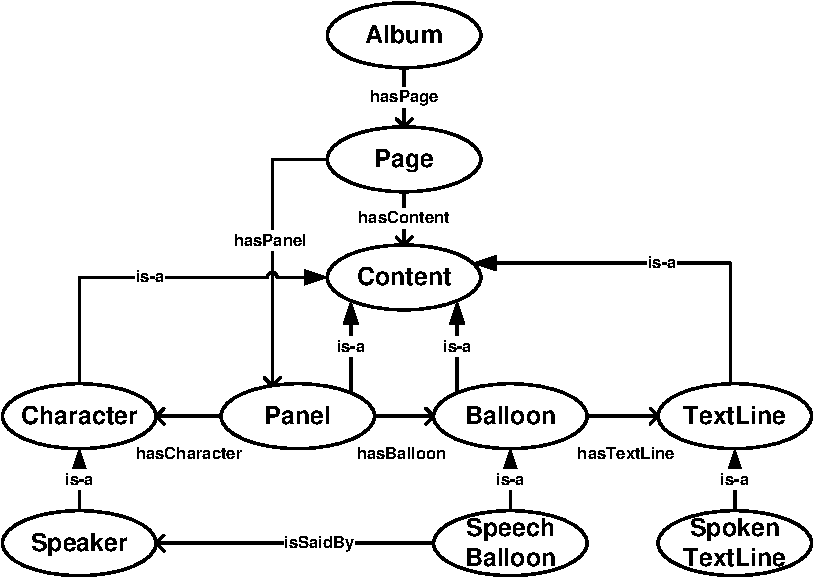
\includegraphics[width=0.7\textwidth]{model_comics.pdf}
  \caption[A representation of the main aspects of the comics model involved in the expert system]{A representation of the main aspects of the comics model involved in the expert system. Concepts are represented by the oval-shaped items, full arrows represent subsumption relations, simple arrows are the object properties linking them to each others. Attributes are not displayed to make it more comprehensible.}
  \label{fig:kn:model_image}
 \end{figure}

\subsection{Model interactions}
The image and comics models are linked through two bridges.
First, the \textit{Image} from the image model and \textit{Page} from the comics model concepts are made equivalent by the axiom \texttt{owl:equivalentClass}.
This way we ensure that all extracted content related to an image is equally related to a corresponding page in the comics domain $Page \equiv  Image$.

Second, the classes $Cl=\{Panel$, $Balloon$, $TextLine$, $Character\}$ are defined as equivalent to the corresponding set of regions of interest $Sr = \{panels$, $balloons$, $text lines$, $characters\}$, see Equation~\ref{eq:kn:class_region_equivalence}.% that have an extractor which purpose is to extract the corresponding panels (resp. balloons, text lines and characters).
	

\begin{equation}
\label{eq:kn:class_region_equivalence}
\begin{split}
Cl_i  \equiv \text{ROI} \textbf{ and } (hasExtractor \textbf{ some } (roiType \textbf{ value } Sr_i ))
\end{split}
\end{equation}

% section model (end)


\section{Interactions between high and low level processing}
\label{sec:kn:interaction_low_high_level_processing}

%This section describes how the extracted data are processed at the semantic level.
This section presents the low and high level processing interaction to validate the extractions, infer information and generate hypotheses about the image content.% we use it to validate the extracted elements, infer more information about them and express region of interest's hypothesis to send back at low-level algorithms.
\subsection{Validation of the extractions} % (fold)
\label{sub:kn:validation}
In order to validate the extraction of the comic page's components, we made sure that the extracted panels, balloons and text lines were in accordance with the knowledge defined in \ref{sec:kn:knowledge_representation}.
%Those which are not consistent with our model are rejected.

Firstly, each item was loaded into the model as it was labelled (page, panel, balloon, text line or comics character) by the low level processing step.
Then, each element was linked to its smallest container in a half-blind way (as defined Section~\ref{sec:kn:knowledge_representation}).
That is to say that the type of contained element was known, while the type of  potential container was not.
Not knowing the type of container might have lead to incorrect assertions that would have produced inconsistencies in the model.
Those inconsistencies are the result of possible mistakes made during the extraction process that were filtered out in order to improve the overall detection precision.
Consistency checking was performed over the model and inconsistencies were handled one after the other.
We chose to focus on increasing the extraction precision by deleting those elements that did not fit the constrained model.
The detection of misclassified elements (a panel actually being a balloon) and the proposition of missed elements (like a missed balloon around a group of text lines) were both perspectives of this work.
For the time being, our system can handled, without being limited to, the following inconsistencies:
%Due to the limited number of object types we deal with, inconsistencies sources can be reduced to this exhaustive list:
\begin{itemize}
	\item \textbf{A page (p) contains a balloon (b), a text line (t) or a character (c)}: b, t or c is deleted.
%	\item \textbf{A page (p) contains a balloon (b)}: if b contains other balloons then b is a panel, otherwise b has to be deleted.
%  	\item \textbf{A page (p) contains a text line (t)}: if t contains other lines then t is a balloon, otherwise t has to be deleted.
	\item \textbf{A panel (p1) contains a panel (p2) or a text line (t)}: p2 or t is deleted.
%  	\item \textbf{A panel (p1) contains a panel (p2)}: if p2 contains any text line then p2 is a balloon, otherwise p2 has to be deleted.
% 	\item \textbf{A panel (p) contains a text line (t)}: if t contains other lines then t is a balloon, otherwise t has to be deleted.
 	\item \textbf{A balloon (b) contains a panel (p)}: if p contains some balloons and b does not contain any text lines, b is deleted, otherwise, p is deleted.
 	%does not contain anything then p is a line, else if p contains any text line then p is a balloon, otherwise b has to be deleted.
	\item \textbf{A balloon (b1) contains a balloon (b2)}: if b1 does not contain any line then b1 is deleted, otherwise b2 is deleted.
	\item \textbf{A balloon (b) contains a character (c)}: c is deleted.
	%\item \textbf{A balloon (b1) contains a balloon (b2)}: if b2 does not contain anything then b2 is a line, else if b1 does not contain any line then b1 is a panel, otherwise b1 has to be deleted.
 	\item \textbf{A text line (t) contains a panel (p)}: if p does not contain any balloon then p is deleted, otherwise t is deleted.
 	\item \textbf{A text line (t) contains a balloon (b)}: if b does not contain any text line then b is deleted, otherwise t is deleted.
	%\item \textbf{A balloon (b1) contains a balloon (b2)}: if b1 does not contain any line then b1 is deleted, otherwise b2 is deleted.
 	\item \textbf{A text line (t1) contains a text line (t2)}: if t1 contains other lines then t1 is deleted, otherwise t2 is deleted.
 	\item \textbf{A text line (t) contains a character (c)}: c is deleted.
 	\item \textbf{A character (c) contains a panel (p), a balloon (b) or a text line (t)}: c is deleted. 	
 	\item \textbf{A character (c1) contains a character (c2)}: c2 is deleted.
\end{itemize}
% subsection validation (end)

\subsection{Inferences from the low level information} % (fold)
\label{sub:inference_from_low_level}

The expert system is able to infer more specific information than that given by the extractors.
For instance, it can deduce which text is spoken or not and which speaking character pronounces the content of which speech balloon.

% % Use of RDFS/OWL (Web ontology language) to model the information domain with the general comics properties listed bellow, base on the type of region given by the low level processing:

% % subsection inference_ (end)

% % \subsection{Region of interest of character (step 4)} % (fold)
% % \label{sub:speaking_region}
% % TO COMPLETE (Clement?)

% The expert system infers the speaking character location from valid speech balloons regions by computing a region from the tail tip to the panel side following the tail direction, for each speech balloon.
% ...
% Those regions are voluntary quite large to maximize the chance to cover at least the speaking characters.

% The regions are passed to the image processing part (character extractor) that will extract all the characters using those regions as seeds.

\paragraph{Speech balloon and speech text} % (fold)
\label{par:speech_balloon_and_speech_text}

The classification of balloons and text respectively into speech balloons and spoken text can be done by running an inference engine on the model (e.g. Racer~\cite{Haarslev2012}] or Pellet~\cite{Sirin2007a}).
To allow reasoning, the model has to be consistent, which is the case after validation step~\ref{sub:kn:validation} when all inconsistencies have been resolved.
In Section~\ref{sec:kn:knowledge_representation}, we defined a speech balloon as a balloon that has a tail.
In others words, the concept of a \textit{speech balloon} can be seen as a specialization of the \textit{balloon} concept that extends all its properties plus adding a few new ones.
This is expressed in the expert system by defining a property \textit{hasTail} with the constraint that must have a \textit{speech balloon} instance as a source.
Assessing this piece of knowledge, the reasoner will automatically deduce that each instance of \textit{balloon} extended with a \textit{hasTail} property can be specialized into a \textit{speech balloon}.

In a similar way, the concept of \textit{text line} subsumes the concept of \textit{spoken text line}.
It is rendered equivalent to the set of individuals from the \textit{text line} concept that is bound with the property \textit{isLineOf}, which is the inverse property of \textit{hasLine}, to a \textit{speech balloon}.
In other words, the text lines marked as being part of a speech balloon are automatically classified as spoken text lines.


\paragraph{Speaking characters} % (fold)
\label{sub:inference_of_the_speaking_characters}
Among the validated characters (see~\ref{sub:kn:validation}), we considered as being potential speakers those who intersect with the hypothetical region computed in \ref{sec:se:tail_to_character}.
These regions were computed from each speech balloon, i.e. the balloons that had an identified tail.
An abstract straight line was drawn from that tail tip in the direction indicated by the tail.
The first region of a potential speaker that it touched was considered to be the source of the speech balloon.
This relation was asserted into the ontology with the property \textit{isSaidBy}, between the selected character and the corresponding balloon.
Since the range of this property was set to the concept of \textit{speaking character}, it automatically classified the character instance involved into this class.

% section interaction_low_high_level_processing (end)


% Conclusion --------------------------------------------------------------------------------------------------------------------------------------
\section{Conclusions}
\label{sec:kn:conclusion}

TODO

In the next chapter, we are going to experiment the different contributions presented in this thesis and compare them to other methods from the literature.
The dataset is first introduced along with the metrics we used to evaluate information retrieval. 

% the first comics image dataset and ground truth publicly available for researchers. It is a selection of hundred pages from more than twenty different albums from America, Japan and Europe.
% The construction of the dataset and ground truth and a quality assessment test are detailed.